% Part: history
% Chapter: set-theory
% Section: limits

\documentclass[../../../include/open-logic-section]{subfiles}

\begin{document}
	
\olfileid{his}{set}{limits}	
	
\olsection{极限的严格定义}
	
如今，解决前述问题的标准方案是摆脱无穷小。具体做法如下。

我们已看到，随着 $\beta$ 越来越小，我们得到的梯度近似也越来越好。确实，当 $\beta$ 任意接近 $0$ 时，$f'(c)$ 的值会“无限趋近”于我们想要的梯度。因此，我们无需考虑 \emph{在} $\beta = 0$ 处会发生什么，而只需考察当 $\beta$ 趋近于 $0$ 时 $f'(c)$ 的\emph{变化趋势}。

如此一来，一般性的挑战就在于：如何严格理解如下形式的断言：

\begin{center}
当 $x$ 趋近于 $c$ 时，$g(x)$ 无限趋近于 $\ell$。
\end{center}

我们可以将其更紧凑地写作：
\[
\lim_{x \rightarrow c}g(x) = \ell.
\]
在 19 世纪，魏尔斯特拉斯 在 柯西 早期工作的基础上，为这个表达式提供了一个完全严格的定义。其核心思想是：通过让 $x$ 足够接近~$c$，我们就能让 $g(x)$ 任意接近~$\ell$。更精确地说，我们规定 $\lim_{x \rightarrow c} g(x) = \ell$ 意为：
\[
(\forall\epsilon > 0)(\exists \delta > 0)\forall x \left(|x - c| < \delta \lif |g(x) - \ell| < \epsilon \right).
\]
这里的竖线表示绝对值。也就是说，当 $x \geq 0$ 时 $|x| = x$，而当 $x < 0$ 时 $|x| =-x$；你可以将\emph{这个}函数表示如下：

\begin{center}
	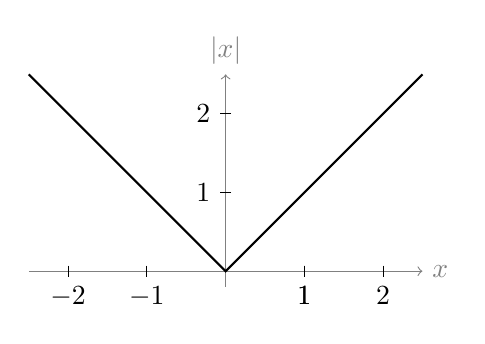
\begin{tikzpicture}[scale=1]
	\draw[->, gray] (-2.5,0) -- (2.5,0) node[right] {$x$};
	\draw[->, gray] (0,-.2) -- (0,2.5) node[above] {$|x|$};
	
	\foreach \x/\xtext in {-2/-2, -1,1, 1/1, 2/2}
	\draw[shift={(\x,0)}] (0pt,2pt) -- (0pt,-2pt) node[below] {$\xtext$};
	
	\foreach \y/\ytext in {1/1, 2/2}
	\draw[shift={(0,\y)}] (2pt,0pt) -- (-2pt,0pt) node[left] {$\ytext$};
	
	\draw[thick] (-2.5, 2.5)--(0,0)--(2.5, 2.5);
	\end{tikzpicture}
\end{center}

所以，这个定义大致是说：通过选取与 $c$ 的距离不超过 $\delta$ 的自变元（即 $|x - c| < \delta$），就能使“误差”小于 $\epsilon$（即 $|g(x) - \ell| < \epsilon$）。

定义了极限的概念之后，我们就能用它来彻底避开无穷小，规定 $f$ 在 $c$ 处的斜率为：
\[
	{f}'(c) = \lim_{x \rightarrow 0}\left(\frac{f(c +x) - f(c)}{x}\right) \text{，其中极限存在}.
\]
不过，重要的是要理解为何我们的定义需要加上“其中极限存在”这一限制条件。举一个简单的例子，考虑我们刚看到的函数 $f(x) = |x|$ 的图像。显然，$f'(0)$ 是未良定义的：如果我们“从右侧”逼近 $0$，斜率总是 $1$；如果我们“从左侧”逼近 $0$，斜率总是 $-1$；因此该极限不存在。鉴于此，我们可以补充定义，函数 $f$ 在 $x$ 处是\emph{可微的}，当且仅当该极限存在。

我们已经看到了如何用\emph{极限}的概念来处理微分。我们还可以用同样的概念来定义\emph{连续}函数的概念。（实际上，波尔查诺 在 1817 年就已经意识到了这一点。）柯西--魏尔斯特拉斯 对连续性的处理如下。粗略地说：一个函数 $f$（在某点）是连续的，前提是：只要对函数的输出有一定的精度要求，就可以通过对函数的输入提出相应的精度要求来保证这一点。更精确地说：$f$ 在 $c$ 处连续，是指当 $x$ 趋于 $0$ 时，$f(c + x)$ 与 $f(c)$ 之差也趋于 $0$。换句话说，$f$ 在 $c$ 处是\emph{连续的}，当且仅当 $f(c) = \lim_{x \rightarrow c} f(x)$。

再深入下去就会偏离到实分析，而我们的主题是集合论。因此，现在我们应该暂停，并总结要旨。在 19 世纪，数学家们学会了如何借助严格定义的\emph{极限}概念来摆脱无穷小。

\end{document}